% ---------------------------------------------------
\chapter{Case Study: Embedded Fault-Tolerant Boot System}
\label{chap:case-study}
% ---------------------------------------------------

\section*{Overview}
This chapter applies the replication and validation techniques from earlier chapters to a concrete embedded target: an ATSAM3X8E (Arduino Due) running a two-stage boot and an RTOS. A Raspberry Pi host automates binary mutation, flashing, boot, and UART log capture. We compare four configurations—Baseline, Majority of 3 (B1+RTOS), Dual Image, and a hybrid \emph{FLCR(B0)+Majority(B1+RTOS)}—under identical fault populations using a repeatable, scripted procedure.

% ---------------------------------------------------
\section{Hardware Testbed}
\label{sec:testbed}

\begin{figure}[t]
  \centering
  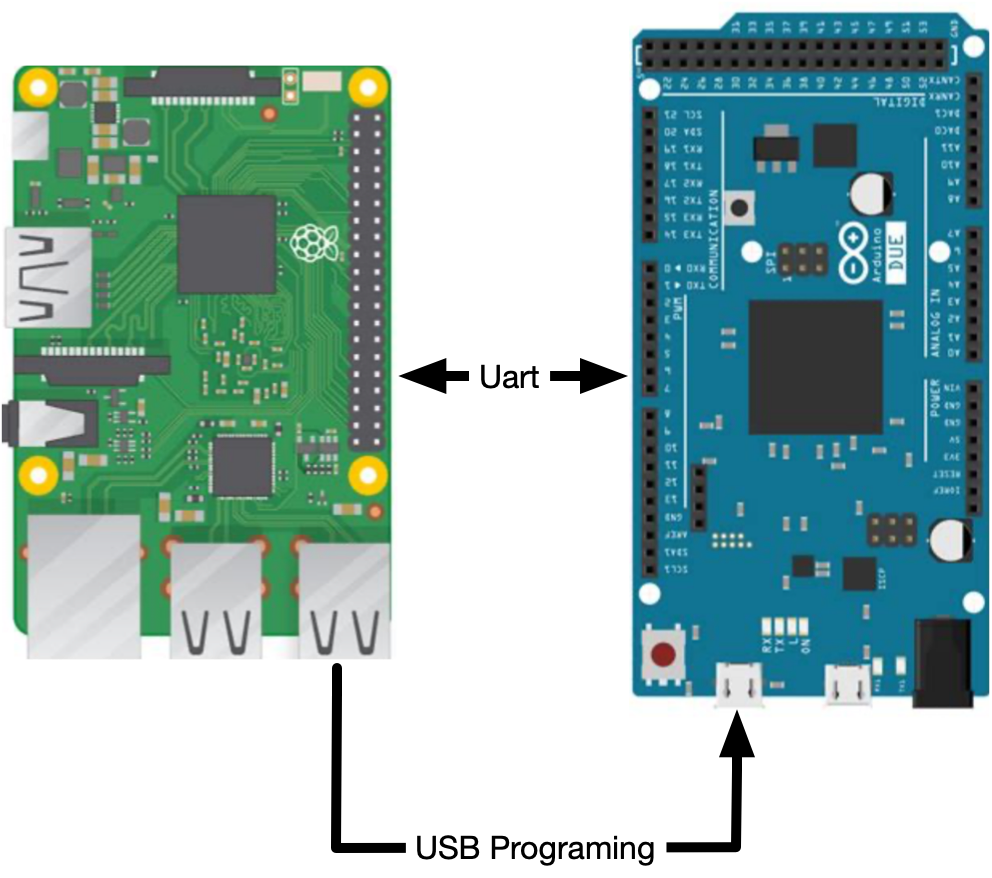
\includegraphics[width=0.85\linewidth]{Chapter-13/figs/test-platform.png}
  \caption{Hardware testbed: Raspberry Pi host (left) and Arduino Due target (right).
  The Raspberry Pi performs binary mutation, flashing, and data collection.
  The Arduino Due executes the boot sequence and returns status and SHA logs over UART.}
  \label{fig:testbed}
\end{figure}

The experimental setup consists of a \textbf{Raspberry Pi 4B} host and an
\textbf{Arduino Due (ATSAM3X8E)} target connected via USB and UART.  
The host manages all experimental control—performing binary mutation,
re-flashing the target, and capturing UART output—while the target executes
the instrumented firmware during each trial.

\paragraph{Host (Raspberry Pi 4B).}
Runs Python-based orchestration scripts on Raspberry Pi OS (64-bit, Debian Bookworm).  
The host coordinates all test automation, including mutation, flashing, log
capture, and SHA verification.

\paragraph{Target (Arduino Due).}
Features an ARM Cortex-M3 @ 84 MHz, with 512 KB of flash (read-only at runtime)
and 96 KB of SRAM (read-write).  
The target executes a two-stage boot sequence (B0 → B1 → RTOS) and reports
the computed SHA digest and status logs over UART.

\paragraph{Connections.}
\begin{itemize}
  \item \emph{USB (programming port)} — reprograms the target using BOSSA.
  \item \emph{UART (USART2 TXD: PD28 / RXD: PD30)} — dedicated link for telemetry and SHA output.
\end{itemize}

This hardware platform enables fully automated, repeatable testing runs,
which are described in detail in the following section.

% ---------------------------------------------------
\section{Evaluation Procedure}
\label{sec:evaluation-proc}

\begin{figure}[t]
  \centering
  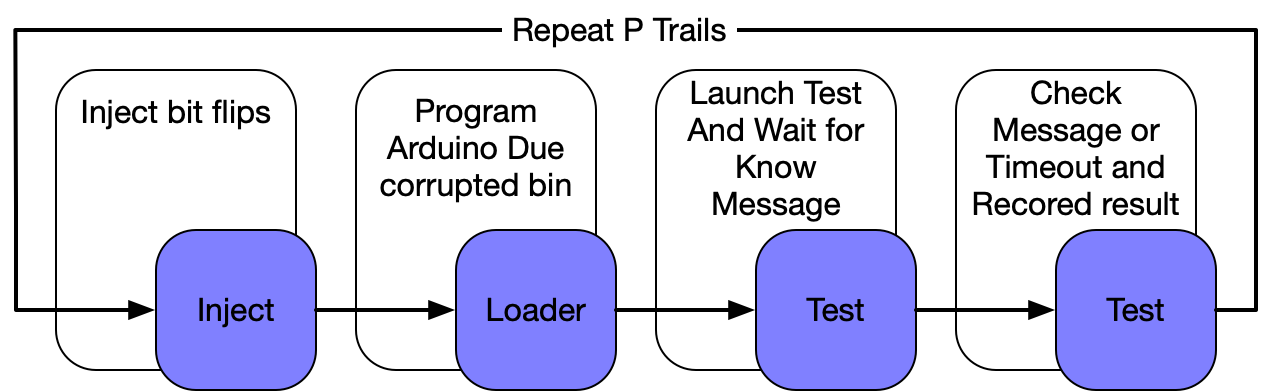
\includegraphics[width=0.9\linewidth]{Chapter-13/figs/test-sequence.png}
  \caption{Automated test sequence. Each iteration injects bit flips into the binary,
  flashes the target, executes the boot sequence, monitors UART output, and records success or failure.}
  \label{fig:test-sequence}
\end{figure}

The evaluation process measures system reliability under randomly injected bit
flips. Each trial executes a complete flash–boot–verify cycle controlled by
the host system. The entire process is automated and repeatable.

\begin{enumerate}
  \item Build the firmware image.
  \item Apply controlled bit flips to the image (fault injection step).
  \item Flash the mutated image to the target via USB.
  \item Boot the target and monitor UART output for SHA or status messages.
  \item Compare the reported SHA digest against the known reference to classify
        the result as \emph{success} or \emph{failure}.
\end{enumerate}

This procedure is repeated for multiple fault densities and random seeds to
capture statistical trends in reliability.

\subsection{Fault Injection}
\label{sec:fault-injection}

Faults are modeled as random bit flips applied directly to the firmware binary \emph{before flashing it to the target}.
Each experiment injects faults at a controlled density determined by the
parameter \(R\) (Bytes with a bit failure). Let \(B\) denote the size (in bytes) of the
tested region of the file.

\paragraph{Expected flips.}
\[
  E \;=\; \left\lceil \frac{B}{R} \right\rceil .
\]

\paragraph{Injection range.}
Bit positions are drawn from the contiguous range
\[
  k \in [\,0,\, E \cdot R \cdot 8\,),
\]
which corresponds to the mutation window of \(E \cdot R\) bytes.
This window is positioned to cover the code under test; only bit indices that
map into the file (\(k < B \cdot 8\)) are eligible. Any index with
\(k \ge B \cdot 8\) is ignored.

\paragraph{Random selection.}
For each trial, draw \(E\) independent integers
\[
  k_1, \dots, k_E \sim \mathrm{Uniform}\{0, \dots, E \cdot R \cdot 8 - 1\},
\]
and toggle the corresponding bits that fall within the file. Duplicate indices
naturally cancel under modulo-2 arithmetic.

\paragraph{Corruption model.}
Let \(X \in \{0,1\}^{B \cdot 8}\) be the original file bitstream; define
\[
  \widetilde{X}
  \;=\;
  X \;\oplus\; \bigoplus_{i=1}^{E} e_{k_i}
  \quad \text{with each term included only if } k_i < B \cdot 8.
\]
The mutated file \(\widetilde{X}\) is then flashed to the target, modeling
persistent (non-volatile) corruption in flash.



% ---------------------------------------------------
\section{System Boot Architecture}
\label{sec:system-boot-architecture}

The embedded system under test follows a two-stage boot architecture that
separates hardware initialization, memory relocation, and runtime execution.
This structure reflects the practical constraints of the ATSAM3X8E
microcontroller, where on-chip flash memory is \emph{read-only at runtime},
requiring executable code to be relocated into SRAM for modification or repair.

\begin{figure}[t]
  \centering
  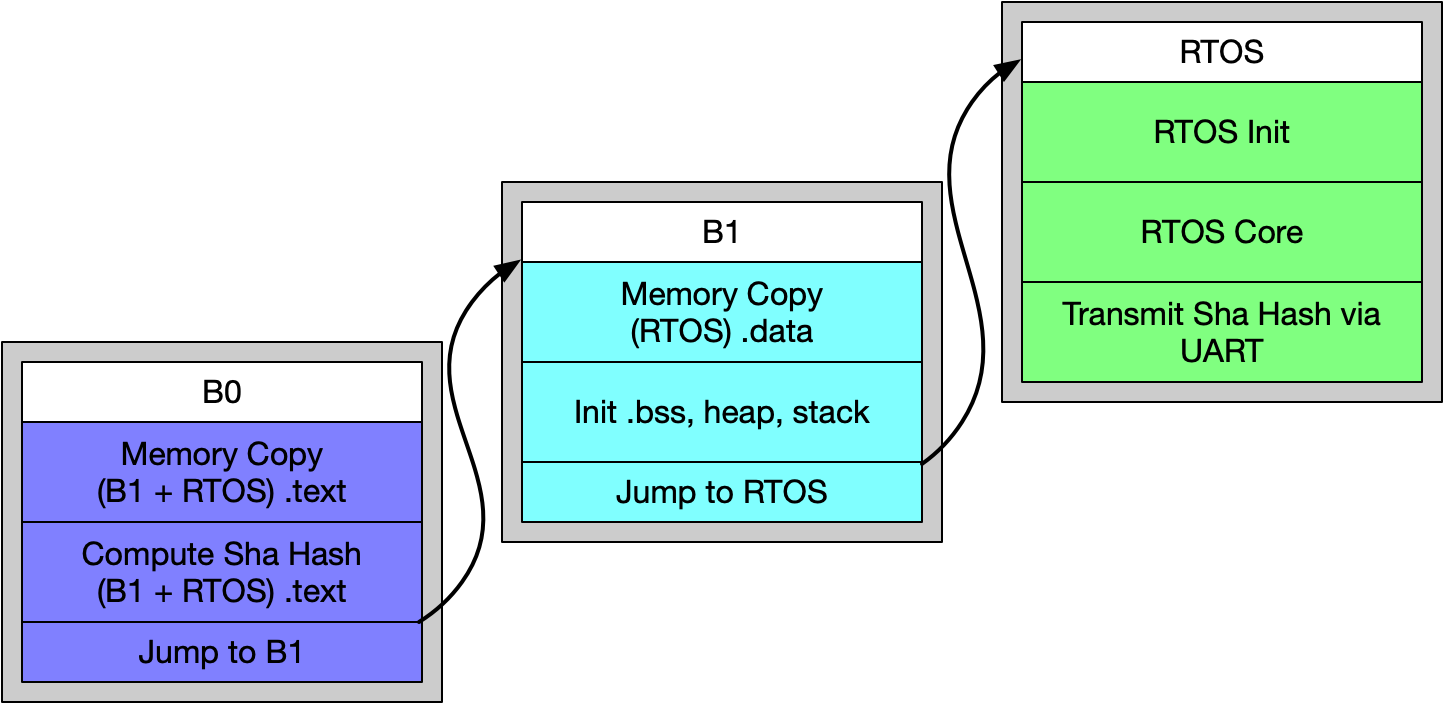
\includegraphics[width=0.95\linewidth]{Chapter-13/figs/boot-overview.png}
  \caption{Two-stage boot sequence showing flash-resident B0 and SRAM-resident
  B1 and RTOS stages. B0 relocates code and computes a SHA digest before
  transferring control to B1, which completes initialization and starts the RTOS.}
  \label{fig:system-boot-architecture}
\end{figure}

\begin{description}
  \item[Stage B0 (Bootloader).]
        Executes directly from flash at reset. B0 performs memory relocation by
        copying all executable sections of B1 and the RTOS (\texttt{.text} and
        \texttt{.rodata}) from flash into SRAM. Once relocation is complete, B0
        computes a SHA digest over the relocated regions and transfers control
        to B1.

  \item[Stage B1 (Application Loader).]
        Executes from SRAM. B1 completes runtime setup by copying
        \texttt{.data} to RAM, initializing \texttt{.bss}, allocating heap and
        stack space, and initializing the relocated vector table. When
        initialization is complete, control transfers to the RTOS initialization
        and kernel runtime.

  \item[RTOS / Runtime.]
        Runs entirely from SRAM. Initializes I/O interfaces and RTOS runtime
        configurations. After startup, the RTOS task begins transmitting the SHA
        digest computed by B0 over UART to the host, enabling the Raspberry Pi
        controller to verify code integrity and record system status.
\end{description}

This two-stage design isolates immutable boot logic (B0) from modifiable
runtime code (B1 and RTOS). Because the CPU cannot modify or write to flash at
runtime, all repair or redundancy mechanisms must operate on the SRAM-resident
images. B0 therefore remains fixed and responsible only for relocation and
validation, while B1 and the RTOS contain the hardened and repairable code
regions evaluated in subsequent sections. The SRAM serves as the writable proxy
for flash. In practice, flash would also be part of the repair domain; however,
its limited program/erase endurance would accelerate cell degradation across
many trials. Thus, performing updates in SRAM accurately models repair behavior
without introducing wear-out artifacts in the hardware.

\section{Basic System Configurations}
\label{sec:basic-configurations}

Two system configurations are evaluated to understand how memory access
restrictions affect the design and effectiveness of fault-tolerant mechanisms.
Both configurations employ an \textbf{Integrity Loader}—a minimal pre-boot
routine that executes before Stage~B0—to increase startup reliability and
establish a verified execution context prior to relocation.

Depending on hardware constraints, the Integrity Loader activates one of two
strategies:
\emph{repair-based hardening}, when writable memory regions are available, or
\emph{replication-based hardening}, when only read-only flash is accessible.
These complementary setups allow evaluation of fault-tolerance under both ideal
and realistic hardware conditions.

% ---------------------------------------------------
\subsection{Scenario A — Writable Flash (Emulated via SRAM)}
\label{sec:scenario-a}

In this configuration, the system emulates a device with writable flash memory,
allowing in-place code repair and recovery during runtime. Although the
ATSAM3X8E microcontroller supports self-programming through the EEFC interface,
repeated program/erase operations during fault-injection campaigns would
\emph{artificially degrade the flash memory}. To preserve device integrity and
enable large-scale experimentation, SRAM is used to \emph{emulate the
effectiveness of updateable flash memory}. All write and repair operations are
redirected to SRAM shadow regions that mirror the flash address layout,
providing an accurate model of in-place repair without incurring physical wear.

\begin{itemize}
  \item \textbf{Integrity Loader.}
        Executes from SRAM before B0. It validates the flash interface and
        initializes the writable SRAM shadow region that serves as a proxy for
        flash. This enables B0 and later stages to perform recovery actions
        as though flash were writable at runtime.

  \item \textbf{B0, B1, and RTOS.}
        All stages execute with writable counterparts mapped into SRAM. During
        recovery, corrupted regions may be repaired by rewriting code or
        metadata within the shadow copy while maintaining the same logical
        structure as flash. Replication can operate alongside repair, forming
        hybrid recovery strategies.

  \item \textbf{Runtime properties.}
        \begin{itemize}
          \item Flash updates are emulated through SRAM shadow regions.
          \item Prevents artificial flash wear during large-scale experiments.
          \item Enables combined evaluation of repair and replication methods.
        \end{itemize}
\end{itemize}

This configuration emulates the operational benefits of having writable flash,
allowing repair-based fault recovery to be tested under conditions equivalent
to a system with full nonvolatile write capability, but without physically
reprogramming flash.


% ---------------------------------------------------
\subsection{Scenario B — Flash Read-Only (Locked System)}
\label{sec:scenario-b}

In this configuration, flash memory is hardware-locked and cannot be modified
while executing. Only SRAM regions are writable, requiring fault recovery to
rely exclusively on replication and redirection rather than in-place repair.

\begin{itemize}
  \item \textbf{Integrity Loader.}
        Executes before B0 to verify that flash contents are consistent and
        readable. Since flash cannot be rewritten, the loader transitions to a
        \emph{replication-based initialization role}, preparing SRAM to receive
        relocated and validated copies of B1 and RTOS code prior to execution.

  \item \textbf{B0, B1, and RTOS.}
        B0 remains fixed in flash and performs relocation only. B1 and RTOS are
        loaded into SRAM, where replication-based hardening (e.g., FLCR or
        majority-voting mechanisms) provides resilience. Fault recovery occurs
        through runtime redirection to verified replicas instead of modification.

  \item \textbf{Runtime properties.}
        \begin{itemize}
          \item Flash is read-only during execution.
          \item Recovery achieved solely through replication and redirection.
          \item Integrity Loader validates flash and initializes replication tables.
        \end{itemize}
\end{itemize}

This configuration reflects the behavior of real embedded systems with
read-only flash, such as the ATSAM3X8E. Here, resilience is achieved entirely
through replication-based mechanisms in SRAM-resident code, isolating runtime
recovery from immutable flash contents.

% ---------------------------------------------------
\subsection*{Configuration Summary}

\begin{table}[h!]
  \centering
  \renewcommand{\arraystretch}{1.15}
  \begin{tabularx}{\linewidth}{|l|c|c|X|}
    \hline
    \textbf{Region} & \textbf{Exec Location} & \textbf{Writable at Runtime} & \textbf{Applicable Techniques} \\ \hline
    \multicolumn{4}{|l|}{\textbf{Scenario A — Flash Fully Writable (Unlocked System)}} \\ \hline
    B0        & Flash/SRAM & Yes & Repair; Replication (FLCR/BBLCR) \\ \hline
    B1, RTOS  & SRAM       & Yes & Repair; Replication (FLCR/BBLCR) \\ \hline
    \multicolumn{4}{|l|}{\textbf{Scenario B — Flash Read-Only (Locked Bootloader)}} \\ \hline
    B0        & Flash & No  & Immutable; validated via SHA \\ \hline
    B1, RTOS  & SRAM  & Yes & Repair; Replication (FLCR/BBLCR) \\ \hline
  \end{tabularx}
  \caption{Runtime writability and hardening capabilities for the two system configurations.}
  \label{tab:system-access-configs}
\end{table}


% ---------------------------------------------------
\section{Protection Domains and Strategy}
\label{sec:protection-domains}

The CPU executes directly from flash at reset, but flash is not writable at runtime; SRAM is writable. This yields two protection domains:
\begin{itemize}
  \item \textbf{Flash (non-writable):} B0 resides/executes here. Fault tolerance uses \emph{replication + redirection} (e.g., FLCR) rather than in-place repair.
  \item \textbf{SRAM (writable):} B1 and RTOS are relocated here. Fault tolerance can use \emph{replication + repair} (e.g., majority voting) on runtime-modifiable code.
\end{itemize}
The configurations below combine these mechanisms across domains.

% ---------------------------------------------------
\section{Test Configurations}
\label{sec:test-configs}

\begin{description}
  \item[Baseline:] No replication or runtime repair; serves as the reference.
  \item[Majority of 3 (B1 + RTOS):] Triplication and majority voting applied to B1 and RTOS (relocated to SRAM); B0 remains baseline.
  \item[Dual Image:] Two complete images in flash; if B0’s SHA check fails on the primary, B0 boots the alternate.
  \item[\( \text{FLCR(B0)} + \text{Majority(B1+RTOS)} \):] B0 uses Function-Level Code Replication (redirection across replicas in flash). B1 and RTOS use Majority-of-3 in SRAM.
\end{description}

% ---------------------------------------------------
\section{Hardened System Overview}
\label{sec:hardened-overview}

Hardening introduces:
\begin{itemize}
  \item \textbf{Boot redirection (B0/flash):} Call sites in B0 resolve through an indirection table populated at startup, allowing control to skip corrupted function copies.
  \item \textbf{Runtime repair (B1+RTOS/SRAM):} Triplicated functions execute under majority voting to mask transient or localized corruption after relocation.
  \item \textbf{Startup ordering:} B0 initializes its redirection metadata before handing off; B1 initializes replicated state and voting logic after relocation.
\end{itemize}

% ---------------------------------------------------
\section{Memory Overview}
\label{sec:memory-overview}

\subsection{Baseline}
\label{sec:memory-baseline}

\begin{figure}[t]
  \centering
  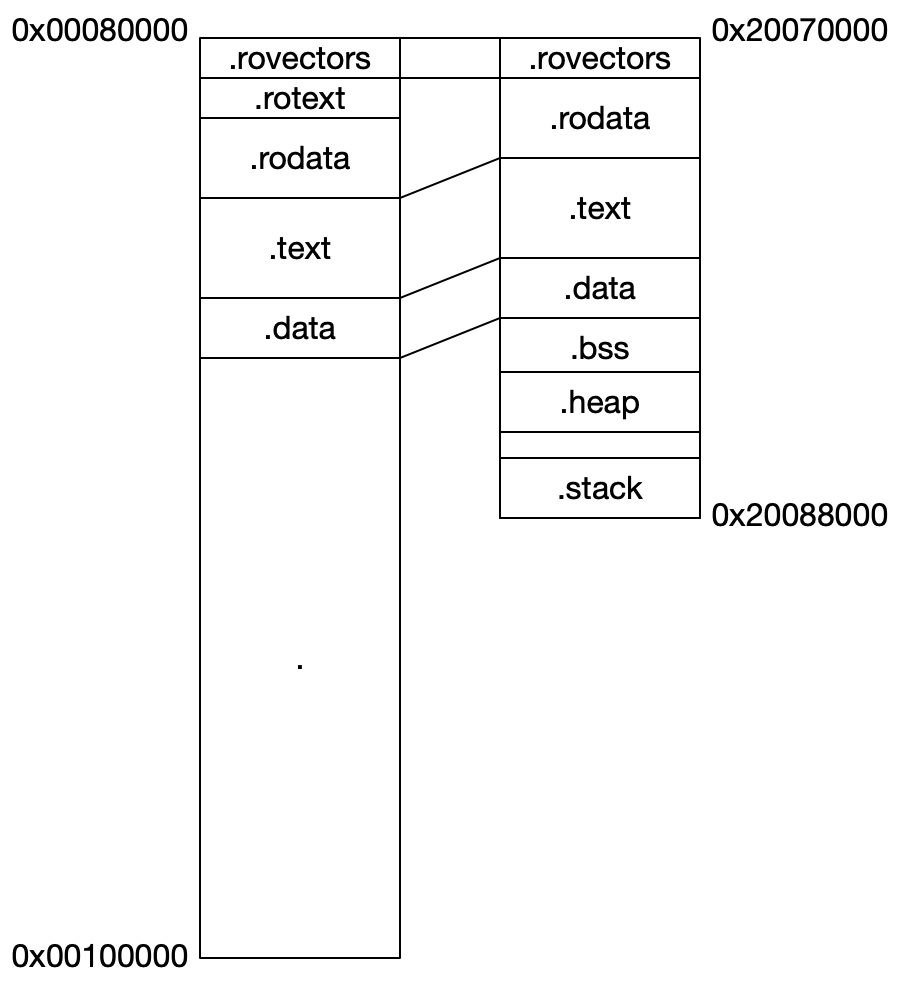
\includegraphics[width=0.72\linewidth]{Chapter-13/figs/baseline-memory.png}
  \caption{Baseline memory layout. At reset B0 copies \texttt{.rovector}, \texttt{.text}, \texttt{.rodata}, \texttt{.data} from flash to SRAM; \texttt{.bss}/heap/stack are created in SRAM; execution proceeds from SRAM.}
  \label{fig:baseline-memory}
\end{figure}

\noindent \textbf{Flash:} persistent copies of \texttt{.rovector}, \texttt{.text}, \texttt{.rodata}, \texttt{.data}. \;
\textbf{SRAM:} relocated code/data plus \texttt{.bss}/heap/stack. \;
No runtime indirection beyond B0’s SHA check.

\subsection{Majority of 3 (B1 + RTOS)}
\label{sec:memory-maj}
B1 and RTOS \texttt{.text} are relocated to SRAM as three replicas per protected function; voter state and minimal metadata reside in SRAM. Flash holds the single persistent image; only one working set is executed from SRAM.

\subsection{Dual Image}
\label{sec:memory-dual}
Flash stores two full images (primary/alternate). B0 executes from flash, validates the selected image, and relocates that image’s \texttt{.text}/\texttt{.data} to SRAM. Only one image is active in SRAM at a time.

\subsection{\( \text{FLCR(B0)} + \text{Majority(B1+RTOS)} \)}
\label{sec:memory-hybrid}
B0 executes from flash with function replicas present in flash and an indirection table/metadata initialized at startup. B1+RTOS relocate to SRAM with triplicated functions and voter logic resident in SRAM. This combines flash-domain redirection with SRAM-domain repair.

% ---------------------------------------------------
\section{Results (placeholder)}
\label{sec:results}
% (Insert reliability curves, overhead tables, and failure-mode histograms.)

\textbf{Planned outputs:} \(\rho(R)\) vs.\ \(R\) for all configurations; boot time and RAM/flash overheads; failure classifications (boot fail / wrong SHA / hang).

% ---------------------------------------------------
\section{Summary}
\label{sec:case-summary}
We defined a consistent hardware automation loop, embedded baseline, and hybrid protection strategy driven by memory writability. Four configurations—Baseline, Majority(B1+RTOS), Dual Image, and \(\text{FLCR(B0)}+\text{Majority(B1+RTOS)}\)—are tested under identical, randomized fault populations using a repeat-\(P\) procedure. Results (next draft) will compare reliability and overhead trade-offs across these approaches.